%%%%%%%%%%%%%%%%%%%%%%%%%%%%%%%%%%%%%%%%%%%%%%%%%%%%%%%%%%%%%%%%%%%%%%%

\chapter{Исследовательские испытания}

%%%%%%%%%%%%%%%%%%%%%%%%%%%%%%%%%%%%%%%%%%%%%%%%%%%%%%%%%%%%%%%%%%%%%%%

\section{Испытания АПК}
Для проверки работоспособности изготовленного образца АПК сбора параметров прототип был установлен в серверную стойку лаборатории "НИЛ АСПОД" в СПБПУ. Методика исследовательских испытаний предполагает сбор климатических параметров в течение чуть больше чем 50 часов. Результаты испытаний описаны ниже.
 
\begin{table}
	\captionsetup{skip=5pt}
	\caption{Результаты мониторинга параметров с использованием АПК}
	\centering
	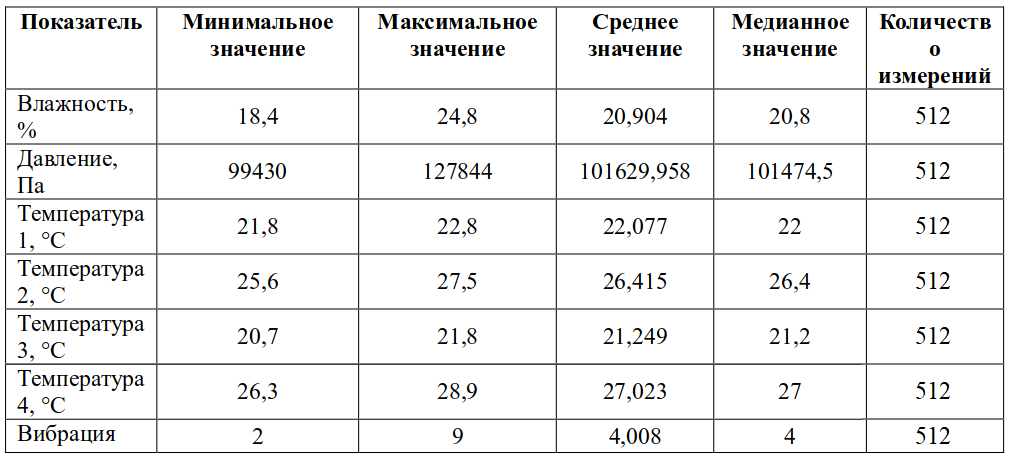
\includegraphics[width=\textwidth]{resultTable}
	\label{tab:result}
\end{table}

Характер  изменения влажности  за  весь  период  наблюдения  приведен  на  рисунке~\ref{fig:humid}.

\begin{figure}[h]
	\centering
	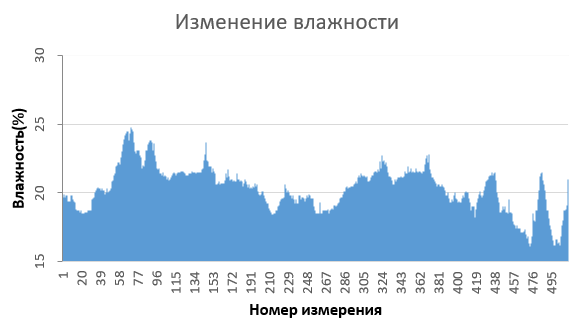
\includegraphics[width=\textwidth]{humid}
	\caption{График изменения влажности за весь период наблюдения}
	\label{fig:humid}
\end{figure}

Изменение  атмосферного давления  на протяжении периода мониторинга приведено на рисунке~\ref{fig:press}

 \begin{figure}[h]
 	\centering
 	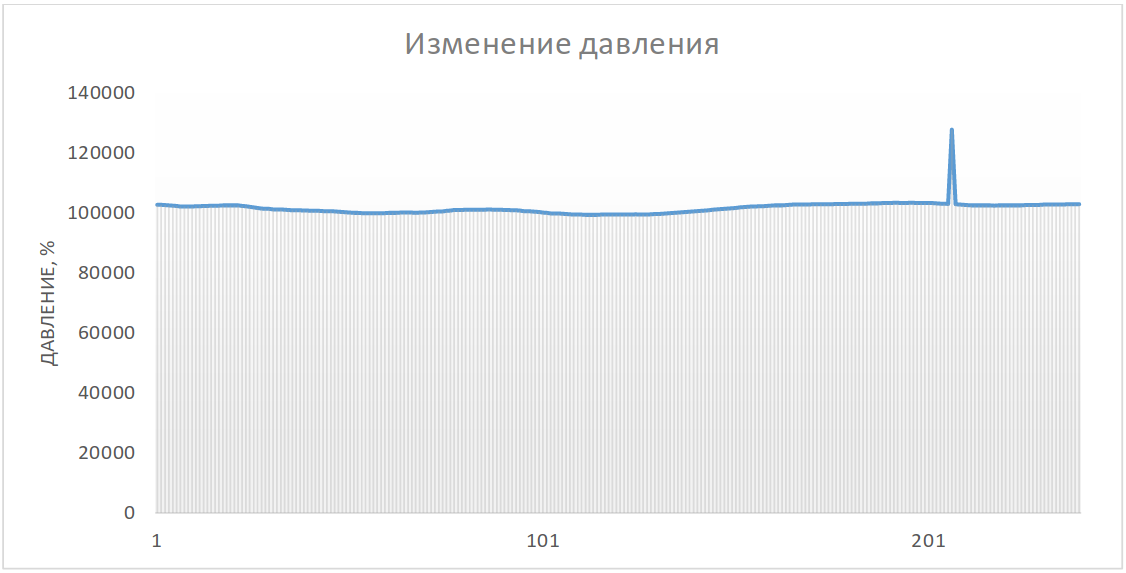
\includegraphics[width=\textwidth]{press}
 	\caption{График изменения атмосферного давления за весь период наблюдения}
 	\label{fig:press}
 \end{figure}

Датчики  температуры  располагались  симметрично  на  передней  и задней стенках серверной стойки сверху и снизу блока.Наибольшая  температура  наблюдается  на  задней  стенке  стойки,  при этом датчики, расположенные сверху задней стенки блока, также показывают большее  значение.  Изменение  температуры  на  протяжении  периода 
мониторинга приведено на рисунке~\ref{fig:temp}.

\begin{figure}[h]
	\centering
	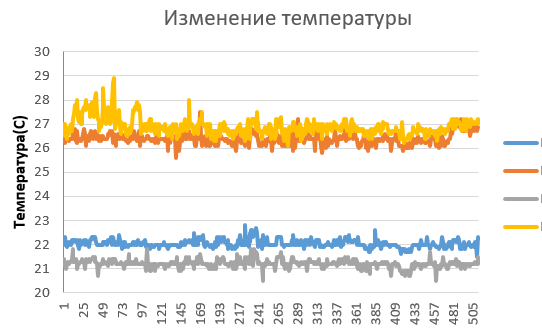
\includegraphics[width=\textwidth]{temper}
	\caption{Объединенный график изменения температуры за весь период наблюдения}
	\label{fig:temper}
\end{figure}

Вибрация  измерялась  как  интегрированное  значение  амплитуды колебаний за последние 100 мс до момента измерения